\documentclass[12pt]{report}
\usepackage[utf8]{inputenc}
\usepackage[russian]{babel}
%\usepackage[14pt]{extsizes}
\usepackage{listings}
\usepackage{graphicx}
\usepackage{amsmath,amsfonts,amssymb,amsthm,mathtools} 
\usepackage{pgfplots}
\usepackage{filecontents}
\usepackage{float}
\usepackage{comment}
\usepackage{indentfirst}
\usepackage{eucal}
\usepackage{enumitem}
%s\documentclass[openany]{book}
\frenchspacing

\usepackage{indentfirst} % Красная строка

\usetikzlibrary{datavisualization}
\usetikzlibrary{datavisualization.formats.functions}

\usepackage{amsmath}


% Для листинга кода:
\lstset{ %
	language=c,                 % выбор языка для подсветки (здесь это С)
	basicstyle=\small\sffamily, % размер и начертание шрифта для подсветки кода
	numbers=left,               % где поставить нумерацию строк (слева\справа)
	numberstyle=\tiny,           % размер шрифта для номеров строк
	stepnumber=1,                   % размер шага между двумя номерами строк
	numbersep=5pt,                % как далеко отстоят номера строк от подсвечиваемого кода
	showspaces=false,            % показывать или нет пробелы специальными отступами
	showstringspaces=false,      % показывать или нет пробелы в строках
	showtabs=false,             % показывать или нет табуляцию в строках
	frame=single,              % рисовать рамку вокруг кода
	tabsize=2,                 % размер табуляции по умолчанию равен 2 пробелам
	captionpos=t,              % позиция заголовка вверху [t] или внизу [b] 
	breaklines=true,           % автоматически переносить строки (да\нет)
	breakatwhitespace=false, % переносить строки только если есть пробел
	escapeinside={\#*}{*)}   % если нужно добавить комментарии в коде
}


\usepackage[left=2cm,right=2cm, top=2cm,bottom=2cm,bindingoffset=0cm]{geometry}
% Для измененных титулов глав:
\usepackage{titlesec, blindtext, color} % подключаем нужные пакеты
\definecolor{gray75}{gray}{0.75} % определяем цвет
\newcommand{\hsp}{\hspace{20pt}} % длина линии в 20pt
% titleformat определяет стиль
\titleformat{\chapter}[hang]{\Huge\bfseries}{\thechapter\hsp\textcolor{gray75}{|}\hsp}{0pt}{\Huge\bfseries}


% plot
\usepackage{pgfplots}
\usepackage{filecontents}
\usetikzlibrary{datavisualization}
\usetikzlibrary{datavisualization.formats.functions}

\begin{document}
	%\def\chaptername{} % убирает "Глава"
	\thispagestyle{empty}
	\begin{titlepage}
		\noindent \begin{minipage}{0.15\textwidth}
			
\includegraphics[width=\linewidth]{img/b_logo}
		\end{minipage}
		\noindent\begin{minipage}{0.9\textwidth}\centering
			\textbf{Министерство науки и высшего образования Российской Федерации}\\
			\textbf{Федеральное государственное бюджетное образовательное учреждение высшего образования}\\
			\textbf{~~~«Московский государственный технический университет имени Н.Э.~Баумана}\\
			\textbf{(национальный исследовательский университет)»}\\
			\textbf{(МГТУ им. Н.Э.~Баумана)}
		\end{minipage}
		
		\noindent\rule{18cm}{3pt}
		\newline\newline
		\noindent ФАКУЛЬТЕТ $\underline{\text{«Информатика и системы управления»}}$ \newline\newline
		\noindent КАФЕДРА $\underline{\text{«Программное обеспечение ЭВМ и информационные технологии»}}$\newline\newline\newline\newline\newline
		
		\begin{center}
			\noindent\begin{minipage}{1.1\textwidth}\centering
				\Large\textbf{  Отчет по лабораторной работе №2}\newline
				\textbf{по дисциплине <<Математическая статистика>>}\newline\newline\newline\newline
			\end{minipage}
		\end{center}
		
		\noindent\textbf{Тема} $\underline{\text{Интервальные оценки~~~~~~}}$\newline\newline
		\noindent\textbf{Студент} $\underline{\text{Нгуен Фыок Санг~~~~~~~~~~~~}}$\newline\newline
		\noindent\textbf{Группа} $\underline{\text{ИУ7-66Б~~~~~~~~~~~~~~~~~~~~~}}$\newline\newline
		\noindent\textbf{Оценка (баллы)} $\underline{\text{~~~~~~~~~~~~~~~~~~~}}$\newline\newline
		\noindent\textbf{Преподаватель} $\underline{\text{Саркисян П. С.}}$\newline\newline\newline
		
		\begin{center}
			\vfill
			Москва~---~\the\year
			~г.
		\end{center}
	\end{titlepage}

\chapter*{Задание}

\section*{Цель работы}
Построение доверительных интервалов для математического ожидания и дисперсии нормальной случайной величины.

\section*{Постановка задачи}

\begin{enumerate}
	\item Для выборки объема $n$ из нормальной генеральной совокупности $X$ реализовать в виде программы на ЭВМ
	\begin{enumerate}
		\item вычисление точечных оценок $\hat\mu(\vec X_n)$ и $S^2(\vec X_n)$ математического ожидания $MX$ и дисперсии $DX$ соответственно;
		\item вычисление нижней и верхней границ $\underline\mu(\vec X_n)$, $\overline\mu(\vec X_n)$ для $\gamma$-доверительного интервала для математического ожидания $MX$;
		\item вычисление нижней и верхней границ $\underline\sigma^2(\vec X_n)$, $\overline\sigma^2(\vec X_n)$ для $\gamma$-доверительного интервала для дисперсии $DX$;
	\end{enumerate}
	\item вычислить $\hat\mu$ и $S^2$ для выборки из индивидуального варианта;
	\item для заданного пользователем уровня доверия $\gamma$ и $N$ – объёма выборки из индивидуального варианта:
	\begin{enumerate}
		\item на координатной плоскости $Oyn$ построить прямую $y = \hat\mu(\vec{x_N})$, также графики функций $y = \hat\mu(\vec x_n)$, $y = \underline\mu(\vec x_n)$ и $y = \overline\mu(\vec x_n)$ как функций объема $n$ выборки, где $n$ изменяется от 1 до $N$;
		\item на другой координатной плоскости $Ozn$ построить прямую $z = S^2(\vec{x_N})$, также графики функций $z = S^2(\vec x_n)$, $z = \underline\sigma^2(\vec x_n)$ и $z = \overline\sigma^2(\vec x_n)$ как функций объема $n$ выборки, где $n$ изменяется от 1 до $N$.
	\end{enumerate}
\end{enumerate}

\chapter*{Теоретические сведения}

\section*{Определение $\gamma$-доверительного интервала для значения параметра распределения случайной величины}

Дана случайная величина $X$, закон распределения которой известен с точностью до неизвестного параметра $\theta$.

Интервальной оценкой с уровнем доверия $\gamma$ ($\gamma$-доверительной интервальной оценкой) параметра $\theta$ называют пару статистик $\underline{\theta}(\vec X), \overline{\theta}(\vec X)$ таких, что

\begin{equation*}
	P\{\underline{\theta}(\vec X)<\theta<\overline{\theta}(\vec X)\}=\gamma
\end{equation*}

Поскольку границы интервала являются случайными величинами, то для различных реализаций случайной выборки $\vec X$ статистики $\underline{\theta}(\vec X), \overline{\theta}(\vec X)$ могут принимать различные значения.

Доверительным интервалом с уровнем доверия $\gamma$ ($\gamma$-доверительным интервалом) называют интервал $(\underline{\theta}(\vec x), \overline{\theta}(\vec x))$, отвечающий выборочным значениям статистик $\underline{\theta}(\vec X), \overline{\theta}(\vec X)$.

\section*{Формулы для вычисления границ \\ $\gamma$-доверительного интервала для математического ожидания и дисперсии нормальной случайной величины}

Формулы для вычисления границ $\gamma$-доверительного интервала для математического ожидания:

\begin{equation}
\underline\mu(\vec X_n)=\overline X + \frac{S(\vec X)t^{St(n-1)}_{\frac{1-\gamma}{2}}}{\sqrt{n}}
\end{equation}

\begin{equation}
\overline\mu(\vec X_n)=\overline X + \frac{S(\vec X)t^{St(n-1)}_{\frac{1+\gamma}{2}}}{\sqrt{n}}
\end{equation}

$\overline X$ -- точечная оценка математического ожидания;

$S(\vec X) = \sqrtsign{S^2(\vec X)}$ -- квадратный корень из точечной оценки дисперсии;

$n$ -- объем выборки;

$\gamma$ -- уровень доверия;

$t^{St(n-1)}_{\alpha}$ -- квантиль уровня $\alpha$ распределения Стьюдента с $n - 1$ степенями свободы.

Формулы для вычисления границ $\gamma$-доверительного интервала для дисперсии:

\begin{equation}
\underline\sigma(\vec X_n)= \frac{(n-1)S^2(\vec X)}{t^{\chi^2(n-1)}_{\frac{1+\gamma}{2}}}
\end{equation}

\begin{equation}
\overline\sigma(\vec X_n)= \frac{(n-1)S^2(\vec X)}{t^{\chi^2(n-1)}_{\frac{1-\gamma}{2}}}
\end{equation}

$S^2(\vec X)$ -- точечная оценка дисперсии;

$n$ -- объем выборки;

$\gamma$ -- уровень доверия;

$t^{\chi^2(n-1)}_{\alpha}$ -- квантиль уровня $\alpha$ распределения $\chi^2(n-1)$ с $n - 1$ степенями свободы.


\chapter*{Результаты работы программы}

\section*{Код программы}

\begin{lstlisting}[language=Matlab]
function lab2()
	X = [10.06,8.32,8.50,8.82,6.02,6.44,7.90,7.85,5.90,7.62,8.66,...
	6.38,7.24,8.21,6.82,7.43,6.06,8.21,9.07,5.85,6.72,8.17,...
	8.53,8.68,7.21,8.43,8.77,7.27,5.79,9.78,6.44,7.24,6.83,...
	6.61,7.58,10.15,8.82,7.87,7.35,9.60,5.82,6.65,10.15,6.92,...
	6.77,9.35,6.92,7.76,6.45,7.47,6.99,9.95,7.22,7.38,7.87,...
	6.24,8.00,8.47,7.25,7.03,7.45,6.75,7.37,7.98,9.58,8.91,...
	6.14,8.19,5.07,7.47,7.29,8.78,7.86,7.82,10.09,8.54,7.21,...
	8.57,6.67,9.82,9.26,9.69,8.39,8.26,7.44,6.58,8.45,7.49,...
	7.16,9.17,8.16,8.38,7.60,8.53,6.10,7.39,7.70,8.45,7.73,...
	9.21,8.02,7.62,6.90,9.55,5.73,7.21,6.14,7.54,9.87,8.14,...
	8.16,7.50,7.60,6.25,7.03,7.07,6.61,9.68,7.65,8.32]; 
	
	n = length(X);
	
	gamma = 0.9;
	alpha = (1 - gamma) / 2;
	
	mu = mean(X);
	s2 = var(X);
	
	fprintf('mu^(MX) = %.2f\n', mu);
	fprintf('s2^(DX) = %.2f\n', s2);
	
	mu_up = mu + sqrt(s2 / n) * tinv((1 + gamma) / 2, n - 1);
	mu_down = mu - sqrt(s2 / n) * tinv((1 - gamma) / 2, n - 1);
	
	fprintf('mu up = %.2f\n', mu_up);
	fprintf('mu down = %.2f\n', mu_down);
	
	
	sigma2_up = (n - 1) * s2 / chi2inv((1-gamma)/2, n - 1);
	sigma2_down = s2 .* (n - 1) ./ chi2inv((1 + gamma) / 2, n - 1);
	
	fprintf('sigma2 up = %.2f\n', sigma2_up);
	fprintf('sigma2 down = %.2f\n', sigma2_down);
	
	N = 1 : n;
	
	M = zeros(1, length(N));
	S = zeros(1, length(N));
	
	for i=N
		M(i) = mean(X(1:i));
		S = var(X(1:i));	
	end
	
	M_up = M - sqrt(S ./ N) .* tinv(1 - alpha, N - 1);
	M_down = M + sqrt(S ./ N) .* tinv(1 - alpha, N - 1);
	
	S_up = S .* (N - 1) ./ chi2inv(alpha, N - 1);
	S_down = S .* (N - 1) ./ chi2inv(1 - alpha, N - 1);
	
	figure
	hold on;
	plot([N(1), N(end)], [mu, mu], 'm');
	plot(N, M, 'g');
	plot(N, M_up, 'b');
	plot(N, M_down, 'r');
	grid on;
	hold off;
	
	figure
	hold on;
	plot([N(1), N(end)], [s2, s2], 'm');
	plot(N, S, 'g');
	plot(N, S_down, 'b');
	plot(N, S_up, 'r');
	grid on;
	hold off;
end
\end{lstlisting}

\section*{Результаты расчётов}
\begin{equation*}
	\hat\mu(\vec x_n) = 7.76\\
\end{equation*}

\begin{equation*}
	S^2(\vec x_n) = 1.30\\
\end{equation*}

\begin{equation*}
	\underline\mu(\vec x_n) = 7.59\\
\end{equation*}

\begin{equation*}
	\overline\mu(\vec x_n) = 7.93\\
\end{equation*}

\begin{equation*}
	\underline{S^2}(\vec x_n) = 1.06\\
\end{equation*}

\begin{equation*}
	\overline{S^2}(\vec x_n) = 1.63\\
\end{equation*}

\begin{figure}[h]
	\centering
	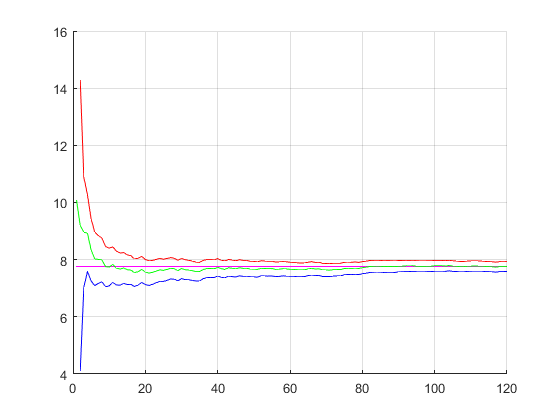
\includegraphics[scale=1]{img/1.png}1
	\caption{Прямая $y(n) = \hat\mu(\vec x_N)$, а также графики функций $y(n) = \underline\mu(\vec x_n)$, $y(n) = \overline\mu(\vec x_n)$, $y(n) = \hat\mu(\vec x_n)$ как функций объема $n$ выборки, где $n$ изменяется от 1 до $N$}
	\label{fig:1}
\end{figure}

\begin{figure}[h]
	\centering
	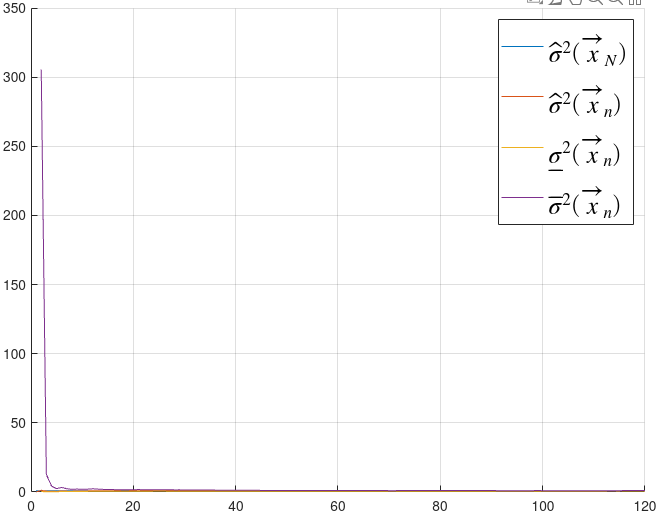
\includegraphics[scale=0.5]{img/2.png}
	\caption{Прямая $z(n) = \hat S^2(\vec x_N)$, а также графики функций $z(n) = \underline S^2(\vec x_n)$, $z(n) = \overline S^2(\vec x_n)$, $z(n) = \hat S^2(\vec x_n)$ как функций объема $n$ выборки, где $n$ изменяется от 1 до $N$}
	\label{fig:2}
\end{figure}

\begin{figure}[h]
	\centering
	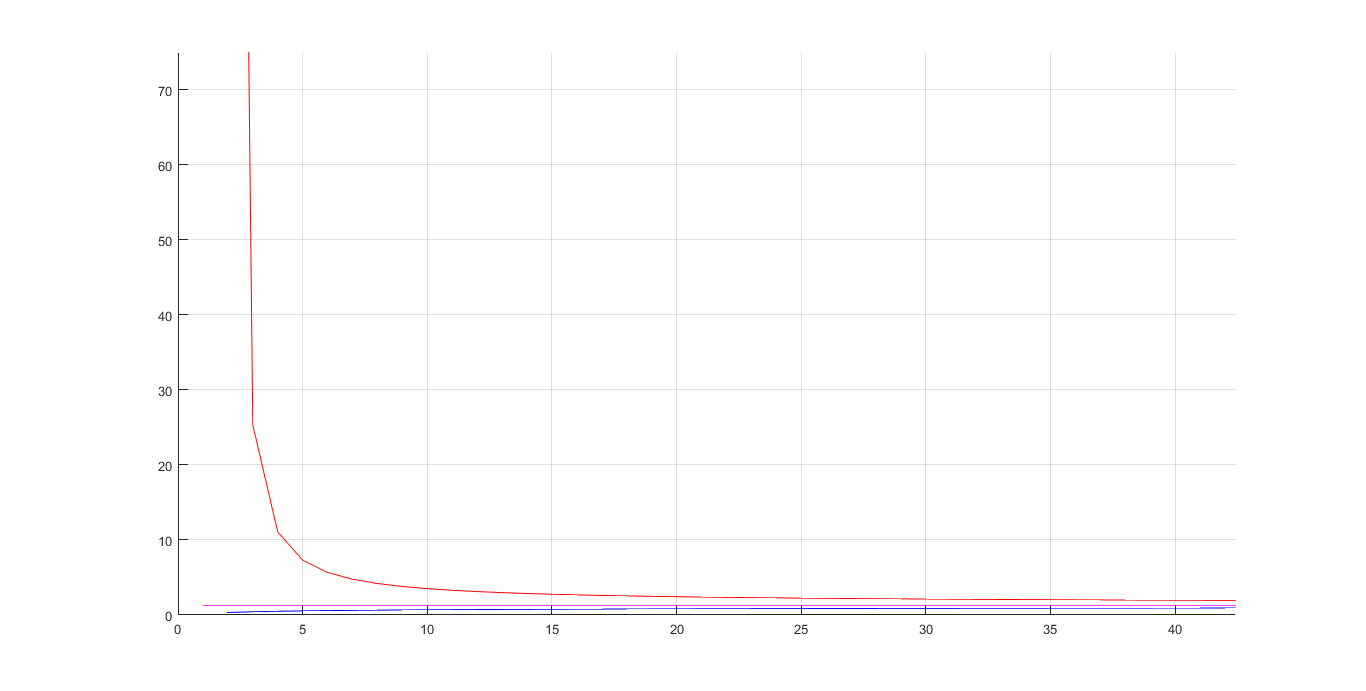
\includegraphics[scale=0.5]{img/3.png}
	\caption{Прямая $z(n) = \hat S^2(\vec x_N)$, а также графики функций $z(n) = \underline S^2(\vec x_n)$, $z(n) = \overline S^2(\vec x_n)$, $z(n) = \hat S^2(\vec x_n)$ как функций объема $n$ выборки, где $n$ изменяется от 1 до $N$ (приближенный)}
	\label{fig:3}
\end{figure}

\bibliographystyle{utf8gost705u}  % стилевой файл для оформления по ГОСТу
\bibliography{51-biblio}          % имя библиографической базы (bib-файла)
	
\end{document}
